\documentclass[12pt]{article}
%\usepackage[utf8]{inputenc}
%\documentclass[UTF8]{ctexart}
%\usepackage[UTF8, heading = false, scheme = plain]{ctex}
\usepackage{geometry}
%geometry{a4paper,scale=0.9}
\geometry{a4paper,left=1cm,right=1cm,top=1cm,bottom=2cm}
\usepackage{amsfonts}
\usepackage{color}
\usepackage{url}
%\usepackage{biblatex}
\usepackage{amsmath}
\usepackage{amssymb}
\usepackage{latexsym}
\usepackage{cite}
%\addbibresource{ref.bib}
%\bibliography{ref.bib}
\usepackage{caption}
\usepackage{graphicx, subfig}
\usepackage{float}
%\usepackage[fontset=ubuntu]{ctex}
%\usepackage{fontspec}
\usepackage{xeCJK}
%\usepackage[colorlinks,
%anchorcolor=black,
%citecolor=black]{hyperref}
%\setmainfont{SimSun}
\usepackage[section]{placeins}
\usepackage{enumitem}
\usepackage{framed}
\usepackage[framemethod=TikZ]{mdframed}
\usepackage{indentfirst}
\usepackage{setspace}%使用间距宏包
\linespread{1.5}
%\title{预备知识}
%\author{leolinuxer }
%\date{June 2020}

\title{分类和回归问题常见的损失函数}
\author{leolinuxer}
%\date{June 2020}

\begin{document}
%\setlength{\parindent}{0pt}
\maketitle
\tableofcontents

\section{损失函数\cite{Compare_Loss_Func_Between_Regression_Classification}}
损失函数一般表示为:$L(y,f(x))$,用来衡量真实值 $y$ 和预测值 $f(x)$ 之间不一致的程度,一般越小越好。为了便于不同损失函数的比较,常将其表示为单变量的函数,在{\color{red}{回归问题中,这个变量为 $y-f(x)$, 在分类问题中,这个变量为 $yf(x)$}}。

\section{回归问题的损失函数}
回归问题中 $y$ 和 $f(x)$ 均为实数 $\in R$,因此用残差 $y-f(x)$ 来度量二者不一致的程度。残差(的绝对值)越大,则损失函数越大,模型效果越差。

\textbf{常见的回归损失函数有:}
\begin{itemize}[itemindent=2em]
    \item 平方损失 (squared loss): $(y-f(x))^2$
    
    \item 绝对值 (absolute loss): $|y-f(x)|$
    
    \item Huber损失 (huber loss): 
    $\begin{cases}
\frac{1}{2}[y-f(x)]^2 & |y-f(x)| <= \delta\\
\delta|y-f(x)|-\frac{1}{2}\delta^2 & |y-f(x)| > \delta\\
\end{cases}$
\end{itemize}

其中最常用的是平方损失,然而其缺点是对于异常点会施以较大的惩罚,因而不够robust。如果有较多异常点,则绝对值损失表现较好,但绝对值损失的缺点是在$y-f(x)=0$处不连续可导,因而不容易优化。

Huber损失是对二者的综合,当$|y-f(x)|$小于一个事先指定的值 $\delta$ 时,变为平方损失,否则是类似绝对值损失。因此也是比较 robust 的损失函数。三者的图形比较如下:
\begin{figure}[ht]
  \centering
  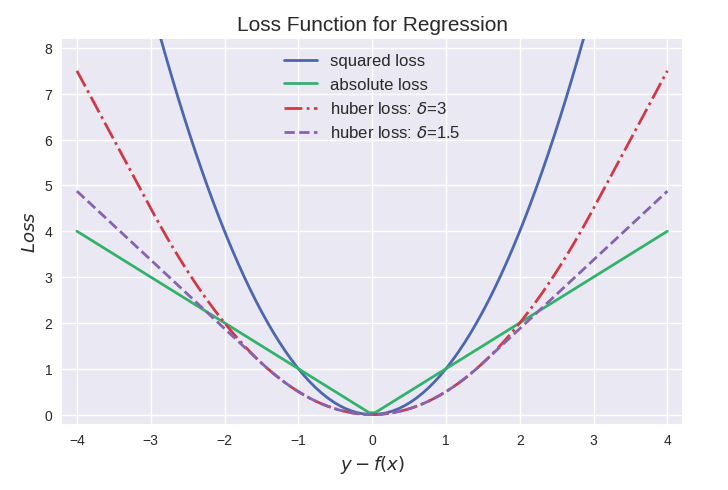
\includegraphics[width=.8\textwidth]{fig/SqureLoss_AbsoluteLoss_HuberLoss_Example.png} %1.png是图片文件的相对路径
  \caption{三种损失函数的示意} %caption是图片的标题
  \label{SqureLoss_AbsoluteLoss_HuberLoss_Example} %此处的label相当于一个图片的专属标志,目的是方便上下文的引用
\end{figure}

\section{分类问题的损失函数}
对于二分类问题 $y\in\{-1,+1\}$,损失函数常表示为关于 $yf(x)$ 的单调递减。如图所示:
\begin{figure}[ht]
  \centering
  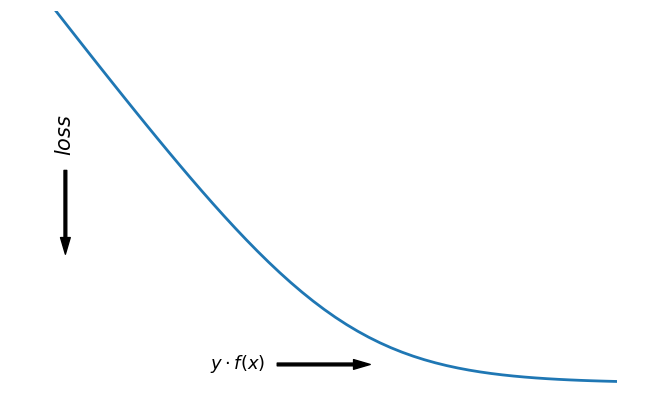
\includegraphics[width=.8\textwidth]{fig/Classification_yfx_example.png} %1.png是图片文件的相对路径
  \caption{分类问题下损失函数 $yf(x)$ 示意图} %caption是图片的标题
  \label{Classification_yfx_example} %此处的label相当于一个图片的专属标志,目的是方便上下文的引用
\end{figure}

$yf(x)$ 被称为\textbf{margin},其作用类似于回归问题中的残差 $y-f(x)$。

二分类问题中的分类规则通常为
$sign(f(x)) = \begin{cases}
+1, & if \quad yf(x) >= 0 \\
-1, & if \quad  yf(x) < 0 \\
\end{cases}$

可以看到如果 $yf(x) > 0$,则分类正确,反之分类错误。\textbf{相应的分类决策边界即为 $f(x) = 0$}。所以最小化损失函数也可以看作是最大化 margin 的过程,任何合格的分类损失函数都应该对 margin<0 的样本施以较大的惩罚。

\subsection{0-1损失(zero-one loss)}
$$L(y,f(x) = \begin{cases}
0, & if \quad yf(x) >= 0 \\
1, & if \quad  yf(x) < 0 \\
\end{cases}$$

0-1损失对每个错分类点都施以相同的惩罚,这样那些“错的离谱“(即 margin $\rightarrow -\infty$)的点并不会收到大的关注,这在直觉上不是很合适。另外0-1损失不连续、非凸,优化困难,因而常使用其他的代理损失函数进行优化。

\subsection{Logistic loss}
$$L(y,f(x)) = \log(1+e^{-yf(x)})$$

Logistic Loss为Logistic Regression中使用的损失函数,下面做一下简单证明:

Logistic Regression中使用了Sigmoid函数表示预测概率:
$$g(f(x)) = P(y=1|x) = \frac{1}{1-e^{-f(x)}}$$

而
$$P(y=-1|x)=1-P(y=1|x)=1-\frac{1}{1-e^{-f(x)}}=\frac{1}{1+e^{f(x)}}=g(-f(x))$$

又因为有$y\in\{-1,+1\}$,所以可以将$P(y|x)$改写为$P(y|x)=\frac{1}{1+e^{-yf(x)}}$,此为一个概率模型,利用极大似然的思想:

$$max(\prod_i^m{P(y_i|x_i)}) = max(\prod_i^m\frac{1}{1+e^{-y_if(x_i)}})$$

两边取对数,又因为是求损失函数,则将极大转为极小:

\begin{equation}
\begin{split}
    max(\sum_i^m\log{P(y_i|x_i)}) = -min(\sum_i^m\log{\frac{1}{1+e^{-y_if(x_i)}}}) \\
=min(\sum_i^m\log({1+e^{-y_if(x_i)}}))  
\end{split}
\end{equation}

这样就得到了Logistic Loss。

\subsubsection{对数似然损失函数}
$$
L(Y,P(Y|X))=-\log{P(Y|X)}
$$

设$p(y=1|x)=p(x),p(y=0|x)=1-p(x)$,隐含条件为:$y_i\in\{0,+1\}$,假设样本是独立同分布的,它们的\textbf{似然函数}就是各样本后验概率连乘:
$$
L(w) = p(y|w,x)= \prod_{i=1}^{N}p(x_i)^{y_i}(1-p(x_i))^{1-y_i}
$$

对应的\textbf{对数似然损失函数}为:
$$
-\log{L(w)} = - \sum_{i=1}^{N}(y_i\log{p(x_i)}+(1-y_i)(\log{(1-p(x_i))}))
$$


\subsubsection{交叉熵损失}
如果$y\in\{-1,+1\}$,定义 $t=\frac{y+1}{2} \in \{0, 1\}$,则极大似然可写为:
$$\prod_i^m(P(t_i=1|x_i))^{t_i}(1-P(t_i=1|x_i))^{1-t_i}$$
两边取对数并转为极小可得:

$$\sum_i^m(-t_i\log{P(t_i=1|x_i)})-(1-t_i)\log((1-P(t_i=1|x_i)))$$

上式被称为交叉熵损失 (cross entropy loss),可以看到在二分类问题中logistic loss和交叉熵损失是等价的,二者区别只是标签$y$的定义不同($y$的取值范围是$\{0,+1\}$还是$\{-1,+1\}$)。

\textbf{简单来说交叉熵是用来计算两个函数或者概率之间的距离,计算的方式也是使用的KL Divergence。在机器学习的世界里面大概可以认为交叉熵和最大似然估计是一回事,如果看到这两个术语应该把他们联系在一起。}

\subsection{Hinge Loss}
$$L(y,f(x))=max(0,1-yf(x))$$

Hinge Loss为svm中使用的损失函数,hinge loss使得 $yf(x) > 1$的样本损失皆为0,由此带来了\textbf{稀疏解},使得svm仅通过少量的支持向量就能确定最终超平面。

Hinge Loss被翻译为“合页损失”,那么合页究竟长啥样?如图,确实有点像hinge loss的形状:
\begin{figure}[ht]
  \centering
  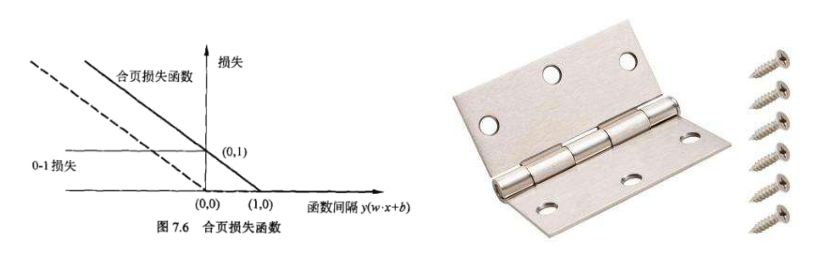
\includegraphics[width=.8\textwidth]{fig/HingeLossExample.png} %1.png是图片文件的相对路径
  \caption{Hinge Loss示意图} %caption是图片的标题
  \label{HingeLossExample} %此处的label相当于一个图片的专属标志,目的是方便上下文的引用
\end{figure}

来看下 hinge loss 是如何推导出来的,带软间隔的svm最后的优化问题可表示为:

\begin{equation}
\begin{split}
    \min_{w,b,\xi}\frac{1}{2}||w||^2+C\sum_{i=1}^m{\xi_i} \\
    s.t. \quad y_i(w^Tx_i+b) >= 1 - \xi_i\\
    \xi_i >= 0, i = 1, 2, \cdots, m\\
\end{split}
\end{equation}

将[2]重新整理有:$\xi_i >= 1 - y_i(w^Tx_i+b)$。若$1 - y_i(w^Tx_i+b)<0$,那么根据约束条件$\xi_i >= 0$,仍然有 $\xi_i >= 0$;若$1 - y_i(w^Tx_i+b)>=0$,则依然为$\xi_i >= 1 - y_i(w^Tx_i+b)$,所以结合之后,可以得到:
$$
\xi_i >= max(0, 1-y_i(w^Tx_i+b)) = max(0, 1-y_i(f(x_i))
$$

取$\xi_i$ 的极小值,即令:$\xi_i=max(0, 1-y_i(f(x_i))$代入目标函数,并令 $\lambda = \frac{1}{2C}$:

\begin{equation}
\begin{split}
    \min{C}\sum_{i=1}^{m}\max{(0, 1-y_if(x_i))} + \frac{1}{2}||w||^2 \\
    \min{\sum_{i=1}^m\underbrace{\max{(0,1-y_i(f(x_i)))}}_{\text{Hinge Loss}}}
     + \lambda||w||^2 \\
\end{split}
\end{equation}

另外可以看到 svm 这个形式的损失函数是自带参数$w$的 $L2$ 正则的,而相比之下Logistic Regression的损失函数则没有显式的正则化项,需要另外添加。

\subsection{指数损失(Exponential loss)}
$$
L(y,f(x))=e^{-yf(x)}
$$

Exponential Loss为AdaBoost中使用的损失函数,使用Exponential Loss能比较方便地利用加法模型推导出AdaBoost算法 (具体推导过程略)。然而其和Squared Loss一样,对异常点敏感,不够robust。

\subsection{Modified Huber Loss}
$$L(y,f(x))= \begin{cases}
\max{(0, 1-yf(x))^2} & if \quad yf(x) >= -1 \\
-4yf(x) & if \quad yf(x) < -1 \\
\end{cases}$$

modified huber loss结合了hinge loss和logistic loss的优点,既能在 $yf(x) >= -1$时产生稀疏解提高训练效率,又能进行概率估计。另外其对于$yf(x)<-1$的样本的惩罚以线性增加,这意味着受异常点的干扰较少,比较robust。scikit-learn中的SGDClassifier同样实现了modified huber loss。

\subsection{全家福}

\begin{figure}[ht]
  \centering
  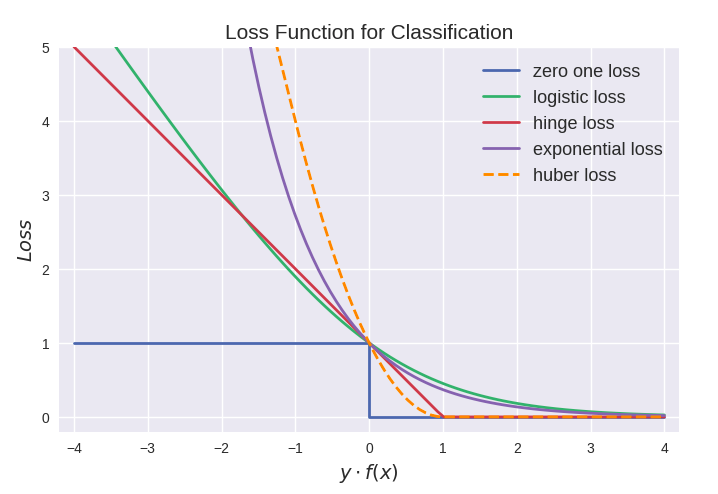
\includegraphics[width=.8\textwidth]{fig/LossFunctionForClassificationOverall.png} %1.png是图片文件的相对路径
  \caption{分类问题的损失函数的全家福} %caption是图片的标题
  \label{LossFunctionForClassificationOverall} %此处的label相当于一个图片的专属标志,目的是方便上下文的引用
\end{figure}

%\printbibliography
\bibliography{../ref}
\bibliographystyle{IEEEtran}
\end{document}
